\section{Smart Home}
\label{sec:smartHome}
    \acl{SH}, im Deutschen \textit{“intelligentes Zuhause“}, ist ein wesentliches Anwendungsgebiet des \acs{IoT}. 
    Diese Rubrik der Anwendung widmet sich überwiegend dem Gebrauch im privaten Umfeld und sämtlichen Haushaltsgeräten 
    und -einrichtungen. Ein kleiner Ausschnitt solcher Nutzgegenstände sind unter anderem Lampen, Kontaktsensoren, 
    Thermostate, Service-Roboter, Staubsauger-Roboter, Kühlschränke Geräte rundum die Haussicherheit. 
    \\ 
    Unter dem Oberbegriff \acl{SH} ist eine Weise zu verstehen, mit der die Erhöhung der Wohn- und Lebensqualität, 
    Energienutzung unter Verwendung vernetzter und fernsteuerbarer Geräten effizienter gestaltet, Sicherheit gesteigert 
    und Abläufe verschiedener Prozessschritte automatisiert werden kann.
    \\ 
    Der Begriff \textit{intelligentes Zuhause} wird verwendet, wenn die Haustechnik und Haushaltsgeräte untereinander 
    vernetzt sind. Die Definition im Deutschen Gebrauch, welche nach (Strese et al. 2010) in der Untersuchung im Rahmen 
    der wissenschaftlichen Begleitung zum Programm Next Generation Media (NGM) des Bundesministeriums für Wirtschaft und 
    Technologie aufgegriffen wird, lautet wie folgt: 
    \begin{quote}
        „Das Smart Home ist ein privat genutztes Heim (z.B. Eigenheim, Mietwohnung), in dem die zahlreichen Geräte der 
        Hausautomation (wie Heizung, Beleuchtung, Belüftung), Haushaltstechnik (wie z.B. Kühlschrank, Waschmaschine), 
        Konsumelektronik und Kommunikationseinrichtungen zu intelligenten Gegenständen werden, die sich an den 
        Bedürfnissen der Bewohner orientieren. Durch Vernetzung dieser Gegenstände untereinander können neue 
        Assistenzfunktionen und Dienste zum Nutzen des Bewohners bereitgestellt werden und einen Mehrwert 
        generieren, der über den einzelnen Nutzen der im Haus vorhandenen Anwendungen hinausgeht.“ \cite{strese.2010m}
    \end{quote}
    Eine vergleichbare Definition wurde zu späterem Zeitpunkt durch eine Literaturrecherche publiziert. Diese beschreibt 
    die zugrundeliegende Thematik weniger aus Anwendersicht sonder widmet sich vielmehr dem System und der Konnektivität. 
    \begin{quote}
        „A smart home is a place with heterogeneous systems to many
        front devices with the support of embedded information and
        communication architectures[...]“ \cite{Balakrishnan2018}
    \end{quote}
    Den beiden Definitionen ist zu entnehmen, dass die Kernaussage eine ähnliche ist, es jedoch in Büchern, Fachartikeln, 
    Publikationen an Universitäten und in den verbreiteten Medien bis heute keine durchgängige Definition gibt. Aus der
    % empirischen 
    einschlägigen Literatur wird ersichtlich, dass viele Synonyme für die Benennung der Thematik verwendet werden, darunter 
    beispielsweise: \cite{strese.2010m}
    \begin{itemize}
        \item Connected Home
        \item Elektronisches Haus
        \item Intelligentes Haus (engl. Smart House)
        \item Smart Living
        \item Home of the Future 
    \end{itemize}
    Eine elementare Information im Zusammenhang zu dieser Arbeit ist, dass die Verwendung des Begriffs \textit{intelligentes Büro} 
    ebenso in den Kontext des \acl{SH} gehört. Hierbei wird lediglich die Räumlichkeit im unternehmerischen Jargon verwendet, 
    die ebenso eine Grundlage für die Verwendung von Komponenten des \acl{SH} bietet. 
    \\
    An dieser Stelle wird deutlich, dass die Verwendung des Begriffs als auch die zugrundeliegenden technischen Verfahren 
    weiträumig einsetzbar sind und deshalb die Begriffsdefinition nicht eindeutig festgehalten werden kann. 
    
    \subsubsection*{Teilsysteme des \acl{SH}}
    \label{subsubsec:teilsystemeSH}
        Der Zentrale Punkt des \acl{SH} ist die Automatisierung häuslicher Prozesse. Dadurch sollen dem Nutzer 
        in vielerlei Hinsicht Aufwände erspart und Informationen zentralisiert angezeigt werden. Die Hausautomatisierung 
        umfasst eine Menge von Teilsystemen. Ein Ausschnitt dieser Teilsysteme ist der folgenden tabellarischen Auflistung zu entnehmen: 
        \begin{table}[hbt!]
            \begin{center}
                \begin{tabular}{| p{3cm} | p{12.75cm} | }
                    \hline
                        \textbf{Segment} & \textbf{Beschreibung} \\
                    \hline
                        Licht & Beleuchtung, Lichtmanagement/Szenarien, Storen/Rollos \\ 
                    \hline
                        Zutritt & Zutrittskontrolle, Klingelanlage, Schlösser, Anwesenheits- und Bewegungserfassung \\ 
                    \hline
                        Überwachung & Technische Alarme: Feuer, Rauch, Gas; Intrusion: Glasbruchmelder, Video; Babyphon, Urlaubswachschutz \\ 
                    \hline
                        Notfall & Sprinkleranlage, unabhängige Stromversorgung, Fluchtwegsystem \\ 
                    \hline
                        Metering & Verbrauchszähler für Strom, Gas, Wasser, Wärme, uvm. \\ 
                    \hline 
                        Konsumelektronik & TV, Internet, Smartphones, Tablets, Spielekonsolen etc. \\
                    \hline
                        Hausgeräte & Kühlschrank, Waschmaschine, Staubsauger, Service-Roboter; Hausgeräte-monitoring, -diagnostik, und -fernbedienung \\
                    \hline
                        Heimlogistik & Einkaufs- und Speiseplanung, häusliche Dienste \\ 
                    \hline
                        Hobby & Haustierversorgung, Aquarienmanagement, etc. \\
                    \hline
                        Mobilität & PKW mit Diagnostik, Navigationssystem mit local based services, Info-/Entertainmentangebote etc. \\ 
                    \hline
                \end{tabular}
            \end{center}
            \caption{Teilsysteme des Smart Home \cite{strese.2010m}}
            \label{tab:teilsysteme}
        \end{table}
        \\
        Ein weiterer wichtiger Anhaltspunkt zum Verständnis der Definition von Smart Home ist die Ausstattung der Komponenten mit Intelligenz und die 
        Vernetzung der Teilsysteme. Dadurch steht als Ziel im Vordergrund weniger die übergeordnete zentrale Steuerung, sondern vielmehr die verteilte 
        Intelligenz, um Aufgaben möglichst autonom (eigenständig) abzuarbeiten. Die dabei erzeugten als auch erforderlichen Daten mit anderen 
        Komponenten des Gesamtsystems auszutauschen, ist ebenso ein vorangestelltes Ziel, welches eine intelligente Umgebung schafft. 
        \\
        Eine mögliche Vernetzung und auch Verwendung solcher Komponenten wird in folgender Abbildung (\ref{pic:szenarien-smarhome}) 
        skizziert. Diese Grafik dient als grobe Übersicht potentieller Anwendungsszenarien, repräsentiert jedoch nicht alle Möglichkeiten der Anwendung. %ist allerdings nicht als vollständig zu interpretieren. 
        \begin{figure}[hbt!]
            \centering
            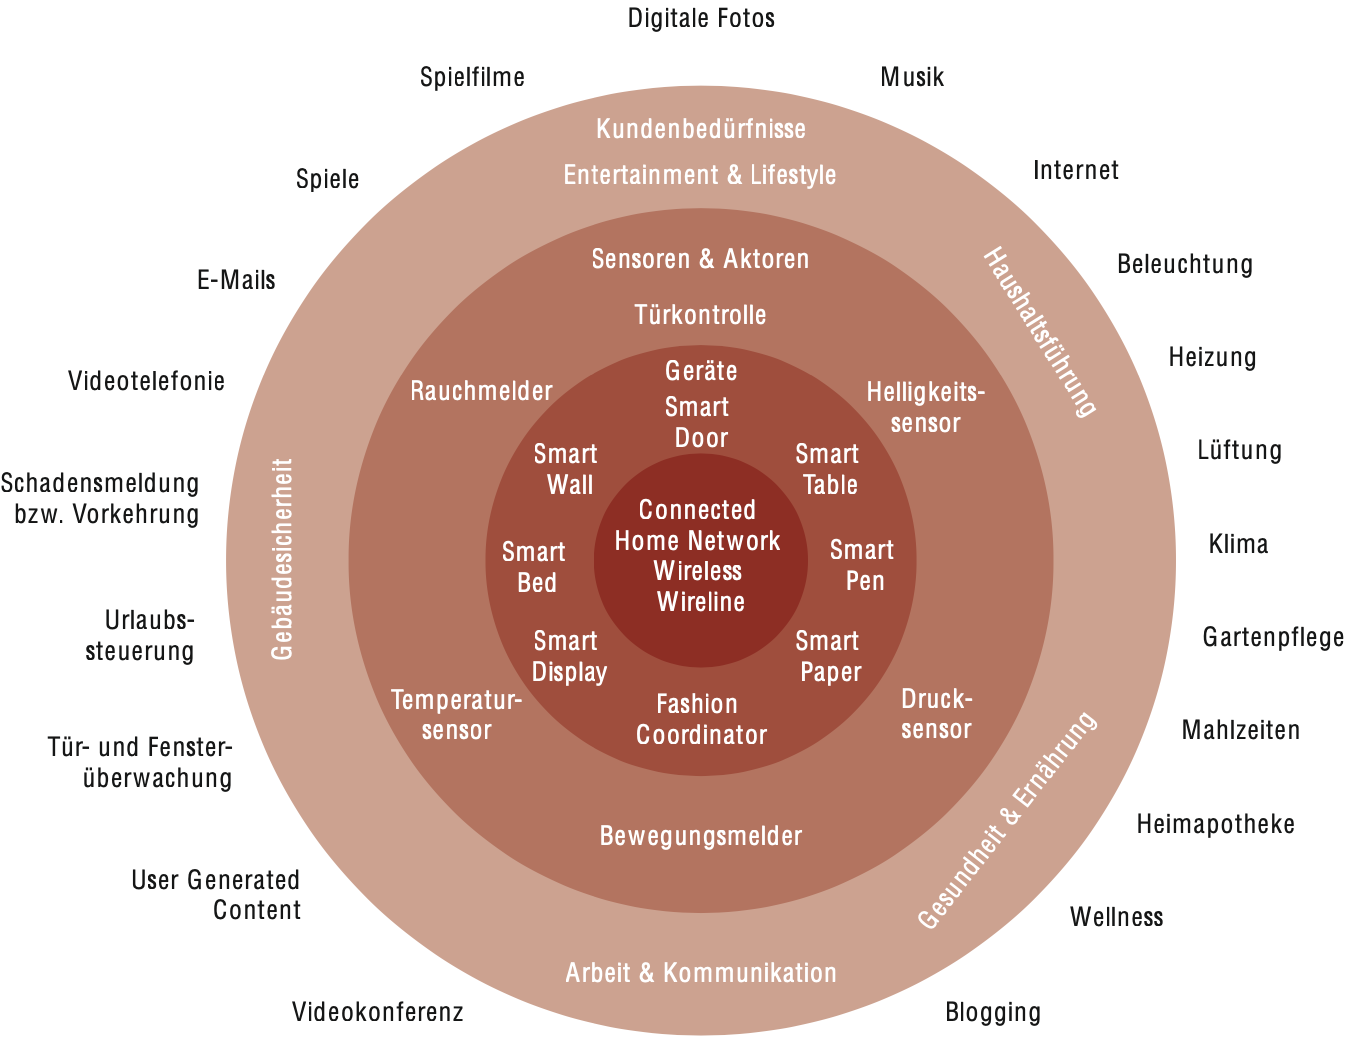
\includegraphics[width=15cm,height=15cm,keepaspectratio]{images/Anwendungsszenarien_SH.png}
            \caption{Mögliche Anwendungsszenarien im Smart Home \cite{strese.2010m}}
            \label{pic:szenarien-smarhome}
        \end{figure}
        \\
        Darüber hinaus gibt es weitaus mehrere Anwendungsszenarien, beziehungsweise werden diese in der Abbildung 
        (\ref{pic:szenarien-smarhome}) in einem Überbegriff zusammengefasst.
        Ein Anwendungsszenario, welches immer mehr Zuwendung findet, ist die Kopplung 
        von Robotern jeglicher Art, darunter Staubsaugerroboter, wobei diese schon weiter verbreitet sind, oder 
        vor allem jedoch Service-Roboter, die immer mehr in die Thematik des \acl{SH} versucht zu integriert werden. 
        
    \subsubsection*{Einordnung von Smart Home in das Internet der Dinge}
    \label{subsubsec:smartHome-IoT}
        Im Konsumentenmarkt wird die Technologie des \acs{IoT} in Produkten eingesetzt, die 
        das Konzept des \acl{SH} verfolgen.  
        Diese beinhalten Haushaltsgeräte und -ausstattung, wie beispielsweise Thermostate, Sensoren, 
        Sicherheitssysteme und Lampen, die mehrere Systeme und Übertragungstechnologien 
        unterstützen. Dazu zählen unter anderem Plattformen, darunter Google Nest, Apple HomeKit 
        und Amazon Alexa uvm. und Übertragungstechnologien, die im Abschnitt (\ref{sec:technologien}) 
        aufgegriffen werden.
        Weitere Beispiele sind der Tabelle (\ref{tab:teilsysteme}) zu entnehmen. 
        \begin{figure}[hbt!]
            \centering
            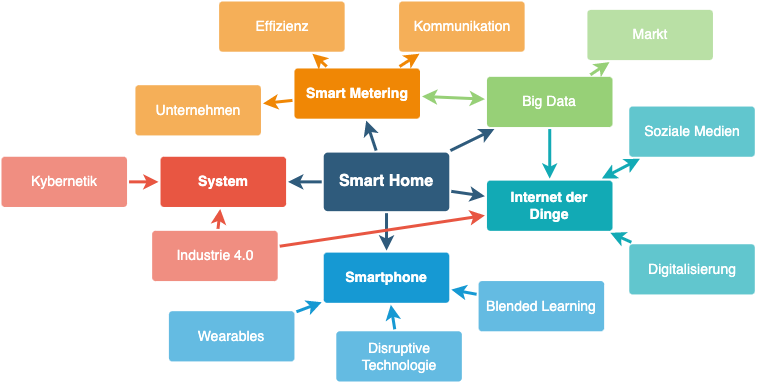
\includegraphics[width=13cm,height=13cm,keepaspectratio]{images/SH-Mind_Map.png}
            \caption{Technologische Einordnung von Smart Home in Verbindung zu IoT \cite{shmindmap2021}}
            \label{pic:mindmap_SH-IoT}
        \end{figure}
        %\\
        %\linebreak
        Die Abbildung (\ref{pic:mindmap_SH-IoT}) zeigt die Verbindungen als auch die Beziehungen von \acl{SH} 
        zu anderen Technologien. Hier wird deutlich, dass im Bereich des \acl{SH} viele Fragestellungen 
        thematisiert werden können, die andere Themenbereiche tangieren. Mit inbegriffen ist zum Beispiel die 
        Komponente Smartphone, da dieses genutzt wird, um als Fernbedienung zu fungieren und Prozesse und 
        Automationen anzeigen und überwachen zu können. Der Bereich des Smart Metering\footnote{Smart Metering ist das computergestützte Messen, Ermitteln und Steuern von Energieverbrauch und -zufuhr. \url{https://wirtschaftslexikon.gabler.de/definition/smart-metering-53998} Abgerufen am 06.04.2022} 
        deckt die Messung von Verbrauchsdaten ab. Dabei handelt es sich um intelligente Messsysteme, die 
        Daten zum Verbrauch, darunter Strom, Gas und Wasser, erheben und diese von den jeweiligen Anbieter zur 
        Rechnungsstellung genutzt werden. Ein Beispiel dazu ist ein digitaler intelligenter Stromzähler mit 
        direkter Kommunikationsmöglichkeit zum Anbieter selbst.
        \\
        \linebreak
        Der Aufbau eines \acl{SH} ist architektonisch ähnlich zu dem Grundprinzip einer \acs{IoT}-Lösung. Die 
        Veranschaulichung des zugrundeliegenden Aufbaus ist der Abbildung (\ref{pic:skizze_iot}) zu entnehmen. 
        \\
        Um die Bezugspunkte zu \acs{IoT} und die Einordnung zu untermauern, wird in folgendem Abschnitt auf 
        die Funktionsweise von \acl{SH} eingegangen. 

    \subsubsection*{Funktionsweise eines \acl{SH}}
    \label{subsubsec:funktionsweise}
        Ein \acl{SH} System besteht aus mehreren Teilsystemen, die in der Regel aus verschiedenen Komponenten bestehen. 
        Wichtige Elemente eines grundlegenden Aufbaus sind die Endgeräte, die sogenannten Aktoren, Eingabegeräte, 
        Sensoren, Gateway und die Vernetzung über Funk, Kabel oder Stromnetz. Die Endgeräte sind die Ausgabegeräte, die 
        über die intelligente Steuerung angesprochen werden können. Darunter zählen zum Beispiel 
        LED-Lampen, Rolläden, Lüftungsanlagen, Lautsprecher, Fernseher, Waschmaschinen und jegliche Arten von 
        Service-Robotern. Eingabegeräte sind die Schnittstelle zwischen der Interaktion des Nutzers und des 
        Smart Home Systems. Das können Wandschalter, Touchdisplays, Fernbedienungen, Smartphones und Regler sein. 
        Mithilfe dieser Schnittstelle können Zustände und Aktionen an den Endgeräten ausgelöst werden. Bei einer 
        fehlenden Verbindung zwischen den Steuerelementen sind diese trotzdem noch über direkte Schaltbefehle möglich. 
        Damit die Zustände ebenso digitalisiert werden können und dem System zur Verfügung stehen, werden Sensoren 
        benötigt. Diese greifen die physikalischen oder elektronischen Eigenschaften des Endgerätes ab, um die 
        Zustände zu ermitteln. Das Gateway repräsentiert die zentrale Steuereinheit, auf dem die Sensordaten 
        eingehen und die Sendung von Befehlen an die Aktoren stattfindet. Ebenso ermöglicht das Gateway die 
        Kommunikation der Endgeräte und Sensoren untereinander. Eine mögliche Internetverbindung zwischen 
        dem Gateway und einer zentralen Plattform, die über die Cloud erreichbar ist, kann ebenso hergestellt werden. 
        Je nach Gerät kann über das Gateway auch eine direkte Steuerung einzelner Elemente stattfinden. Das letzte 
        Element, die Vernetzung, ist dafür zuständig, die Verbindung aller Elemente. Hierfür kommen verschiedene 
        Protokolle, die unter anderem in Abschnitt (\ref{sec:technologien}) beschrieben werden, 
        per Funk, Kabel oder Stromnetz zum Einsatz. % https://www.verbraucherzentrale.de/wissen/umwelt-haushalt/wohnen/smart-home-das-intelligente-zuhause-6882#:~:text=Darunter%20fallen%20zum%20Beispiel%20Heizk%C3%B6rperregler,aus%20einem%20oder%20mehreren%20Eingabeger%C3%A4ten.
        \\
        Ein exemplarischer Aufbau der Komponenten ist der folgenden Abbildung zu entnehmen:
        \begin{figure}[hbt!]
            \centering
            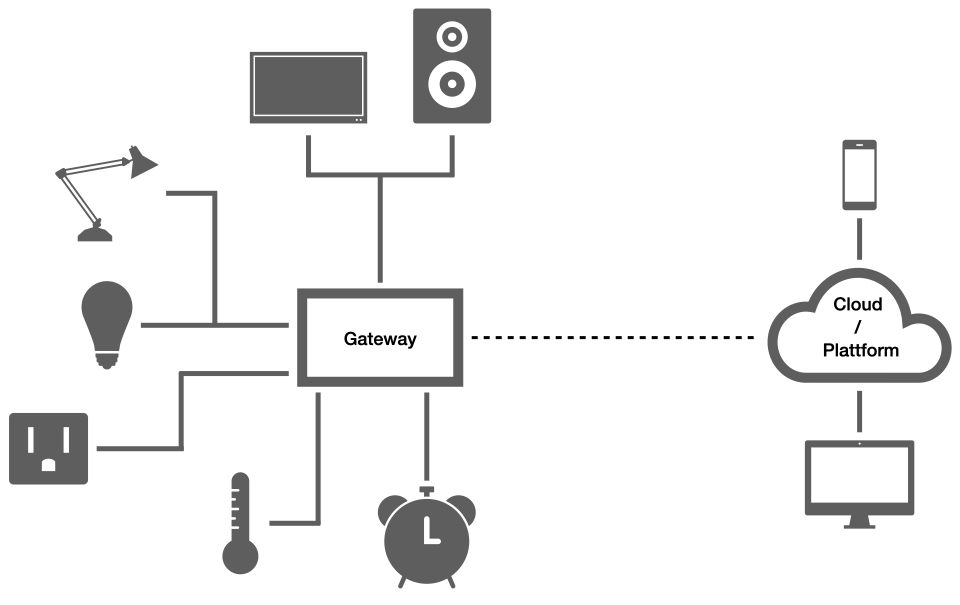
\includegraphics[width=13cm,height=13cm,keepaspectratio]{images/smart_home_connection.png}
            \caption{Aufbau und Funktionsweise einer Smart Home Infrastruktur}
            \label{pic:aufbau_SH}
        \end{figure}

    %\subsubsection{Eigendefinition Smart Home}
    
    \subsection{Historische Entwicklung}
    \label{subsec:entwicklung_sh}
        Im Bereich des \acl{SH} wurde im Jahr 1975 die erste Netzwerktechnologie für Hausautomationen 
        präsentiert und vermarktet. Bekannt wurde diese unter dem Namen \textit{xX0}\footnote{\url{https://de.wikipedia.org/wiki/X10_(Protokoll)} - X10 Protokoll Erklärung. Abgerufen am 06.04.2022}. 
        Dabei handelt es sich um ein stromleistungsbasiertes Netzwerkprotokoll zur Gebäudeautomation. Die 
        Schaltsignale werden über die Hausinstallation, das Stromnetz des Hauses, transportiert. Eingeführt wurde die 
        Technologie von dem Unternehmen Busch-Jaeger unter dem Namen \textit{Timac X10}. Es zeichnete sich durch die 
        einfache Konfiguration und dessen interessanten Funktionen zu diesem Zeitpunkt aus \cite{aschendorf2014energiemanagement}. % URL zur Zitierquelle: https://books.google.de/books?id=-y8pBAAAQBAJ&dq=Bernd+Aschendorf:+Energiemanagement+durch+Geb%C3%A4udeautomation.+Vieweg,+2014,+ISBN+978-3-8348-0573-7,+S.+55.&lr=&hl=de&source=gbs_navlinks_s 
        Die Weiterentwicklung des Systems, Timac X10, fand im Jahre 1998 statt, indem von Busch-Jaeger ein neues 
        Produkt Namens \textit{Powernet EIB} in Deutschland eingeführt wurde. Dieses basierte ebenso auf dem grundlegenden 
        Netzwerkprotokoll X10 und fügte sich nahtlos in den europäischen Installationsbus (EIB/KNX) ein \cite{busch-jaeger}. 
        KNX ist ein Bussystem zur Gebäudeautomation, welches basierend auf dem EIB weiterentwickelt wurde. Es 
        zählt heute noch zu den kabelgebundenen Standards. Im Jahre 2001 eröffnete die Fraunhofer IMS in Kooperation 
        mit der Universität Duisburg-Essen die Fraunhofer-inHaus-Forschungsanlage \cite{fraunhofer-forschungsanlage}. 
        Innerhalb dieser Institution erforschen, entwickeln, testen und demonstrieren Dienstleister, Hersteller und Nutzer 
        mit dem Fraunhofer-Institut und der Universität neue Systemlösungen und weitere Produktkomponenten sämtlicher Arten 
        im Bereich des Wohnens. Anfang des Jahres 2005 wurde die deutsche Telekom in dem \acl{SH} Bereich aktiv und 
        präsentierte der Öffentlichkeit ein vollständig vernetztes „intelligentes“ Musterhaus in Berlin, das sogenannte 
        \textit{T-Com-Haus}. Anfang des Jahres 2012 wurde das \ac{BMWK} im Sektor des \acl{SH} aktiv. Seitdem fördert die 
        Behörde das \textit{„Zertfifizierungsprogramm Smart Home + Building“}, bei dem Forschungen im Bereich des \acl{SH} 
        von Vertretern akademischer Einreichtungen und Industrieunternehmen, die in diesem Segment unterwegs sind, 
        durchgeführt werden. Ziele dabei sind unter anderem die Erstellung von Standards und Prüfsiegeln für 
        systemübergreifende Interoperabilität der Geräte eines \acl{SH} \cite{vde-smartAndBuilding}. 
        2013 bot die deutsche Telekom neue Lösungen in einem weiteren Musterhaus in Darmstadt. 
        Darin sind mehrere Komponenten und Vernetzungen geboten als in dem Vorgänger in Berlin \cite{telekom_SH}. Ein 
        Augenmerk dabei liegt auf der Nutzung verschiedener Funkstandards, die es ermöglichen, intelligente Geräte 
        unterschiedlichster Hersteller zu konfigurieren und über ein Smartphone, Tablet oder Computer zu kontrollieren 
        und steuern \cite{telekom_SH}. Die Auswirkungen der rasanten Entwicklung dieser Technologie treiben das 
        Interesse in die Höhe, sodass 2014 und 2015 die Technologie das Hauptthema der \ac{IFA} bei vielen 
        Ausstellern war.
        \\
        Bis heute wird in dem Segment des \acl{SH} geforscht und immer weitere Funktionalitäten entwickelt. Der Trend 
        der Nutzung von intelligenten Geräten ist weiter zunehmend. Die Marktsituation und der aktuelle Ist-Stand 
        wird in dem Abschnitt Marktanalyse (\ref{sec:marktanalyse}) nochmals aufgegriffen und mit Statistiken und Umfragen belegt.

    \subsection{Ziele von Smart Home}
    \label{subsec:ziele_sh}
        Die Ziele der intelligenten Vernetzung sind in erster Linie die offensichtlichsten, die auch jeweils 
        große Domänen abdecken. Die Ziele sind:
        \begin{itemize}
            \item Komfort (Steuerung, Fernbedienung, Delegation und Automationen)
            \item Energie- und Kosteneffizienz
            \item Sicherheit (Überwachung)
        \end{itemize}
        Allgemein lässt sich der Komfort durch die bequeme Steuerung von Licht, Heizung, Unterhaltungselektronik, 
        Service-Robotern und vielen weiteren Geräten aus der Ferne als auch aus unmittelbarer Nähe steigern. 
        Hierfür spielen beispielsweise Smartphones, zentrale Steuerungsgeräte und Tablets eine wichtige Rolle. 
        Diese fungieren in dem Bezug ähnlich zu einer herkömmlichen Fernbedienung. Es können ebenso Prozesse 
        automatisiert werden oder durch ein bestimmtes vorgegebenes Ereignis, welches 
        eintreten kann, angestoßen werden. Mit diesen Automationen können gewünschte Wohnbedingungen zu 
        bestimmten Anlässen und Zeiten erzeugt werden. Beispielsweise kann die Heizung vor eintreffen höher 
        gestellt werden, damit bei Eintreffen in das Gebäude eine optimale Temperatur herrscht. Die Steuerung von 
        Geräten spielt ebenso eine Rolle in den Bereichen der Energie- und Kosteneffizienz und der Sicherheit. 
        \\
        \linebreak
        Um Energiekosten zu verringern, sind zum Beispiel mehrere Komponenten durch eine Automation miteinander 
        verbunden. Dadurch ist es möglich anhand der Informationen, bspw. des Temperaturfalls bei offenem Fenster 
        anhand von Sensoren zu erkennen, ob ein Fenster offen ist. Dementsprechend kann die Heizung für den Zeitraum 
        ausgeschaltet oder reguliert werden, damit die Heizung nicht überflüssig Wärme erzeugt. Ein weiteres 
        Sparpotential ist das ausschalten von aktuell nicht benötigten Ressourcentypen, wie z.B. Elektrogeräte 
        oder LED-Lampen, die unter anderem vor Verlassen des Gebäudes vergessen wurden auszuschalten.
        \\
        \linebreak
        Das letzte größere Ziel, welches mit \acl{SH} verfolgt wird, ist die Erhöhung der Sicherheit und das Überwachen 
        von Eingängen und Fenstern. So können durch Bewegungsmelder uns Sensoren Aktivitäten registriert 
        werden, die bei Abwesenheit den Eigentümer informieren. Schutz vor Einbruch, bzw. das direkte Handeln auf 
        bestimmte Ereignisse. Mit Kameras können auch Dinge überwacht werden, beispielsweise, wenn ein Haustier 
        kurze Zeit alleine zuhause ist oder Einbruchversuche stattfinden. Ebenso kann eine Alarmierung über Sensoren erfolgen, 
        wenn Wasser im Keller steht oder ein Kurzschluss eines Gerätes ein Feuer auslöst. 
        \\
        \linebreak
        Die Geräte im \acl{SH} erfüllen weitestgehend diese Ziele und werden stetig weiterentwickelt, verbessert und neue 
        Funktionalitäten entwickelt.
